
\section{Introduction}

\begin{frame}
  \frametitle{Whad do we want to achieve?}
    From various sources (HTML, ePub) create PDF suitable for various outputs:
    \begin{itemize}
      \item e-book readers
      \item smartphones or tablets
      \item various print page formats
    \end{itemize}

  \end{frame}
  \begin{frame}
    \frametitle{Why?}

    \begin{itemize}
      \item comfortable reading
      \item archiving
      \item because we can
    \end{itemize}


\end{frame}

\section{Jak zkonvertujeme HTML do PDF pro čtečku?}

\begin{frame}
  \frametitle{Rmodepdf}

  Skript, který zkonvertuje webovou stránku nebo ePub soubor do PDF.

  \begin{itemize}
    \item extrahuje čistý text článků, bez reklam a navigačních elementů na stránkách
    \item měl by umožňovat konfiguraci pro jednotlivé weby nebo vydání e-booků (např. MK Praha)
    \item konfigurovatelný výstup
  \end{itemize}


    
  % Rozpracovaný kód se nachází zde:

    \url{https://github.com/michal-h21/rmodepdf/}
  \end{frame}

\begin{frame}
  \frametitle{Reader mode pro skripty}
  Zobrazení pro čtečku je mód ve webových prohlížečích, který odstraní ovládací prvky ze stránky a zobrazí jen text článku.

  \bigskip

  \begin{tabular}{ll}
    Readability.js & \url{https://github.com/mozilla/readability}\\
    Python-readability & \url{https://github.com/buriy/python-readability}\\
    Rdrview: &\url{https://github.com/eafer/rdrview}\\
  \end{tabular}

\end{frame}

\begin{frame}
  \frametitle{Stránka s ovládacími prvky a reklamami}
  \begin{center}
    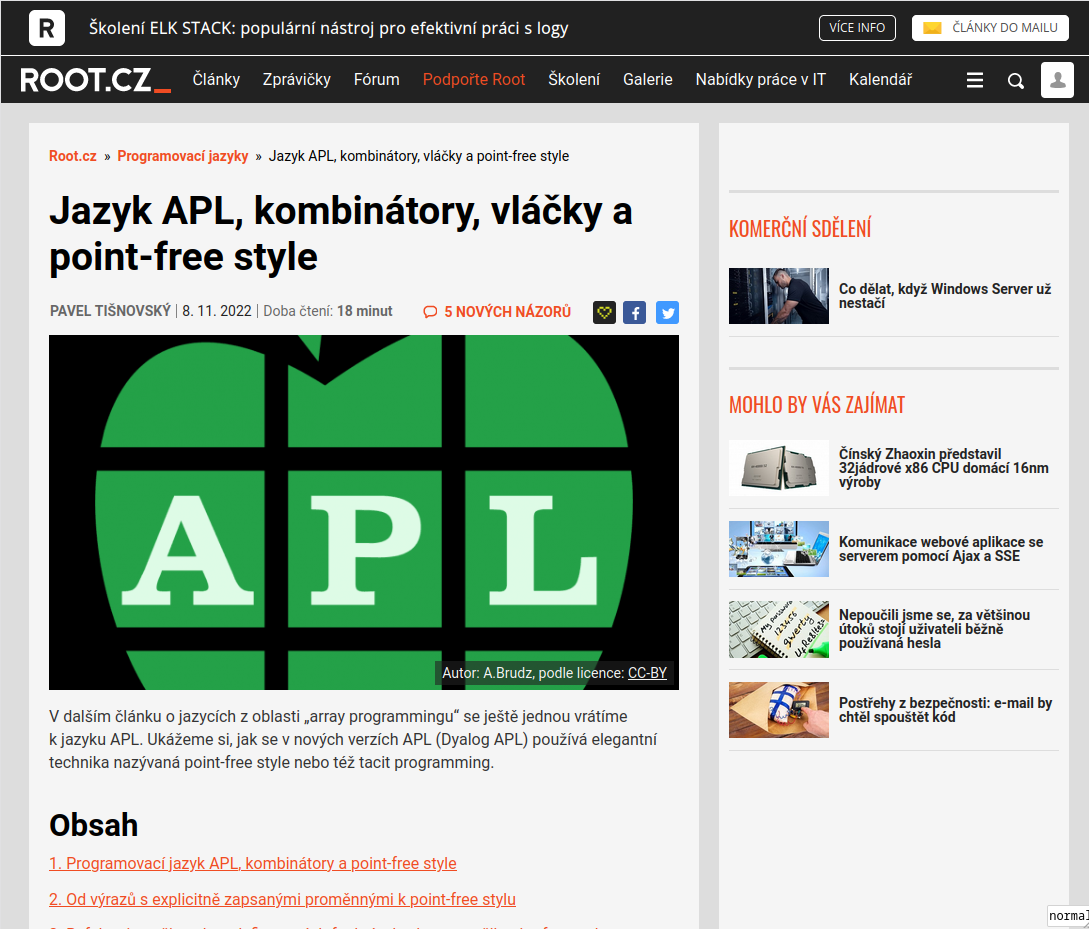
\includegraphics[height=.9\textheight]{img/root-balast.png}
  \end{center}
\end{frame}

\begin{frame}
  \frametitle{Stránka v zobrazení čtečky}
  \begin{center}
    \includegraphics[height=.9\textheight]{img/root-čtečka.png}
  \end{center}
\end{frame}

\begin{frame}
  \frametitle{Jak načteme HTML a ePub soubory?}
  V Lua\TeX u máme několik nástrojů
  \begin{itemize}
    \item knihovna pro čtení ZIP souborů
    \item LuaXML obsahuje knihovnu Transform pro převod XML do jiných formátů, například \TeX u
      \begin{itemize}
        \item umožňuje pravidla pro specifické elementy vybrané pomocí CSS selektorů
      \end{itemize}
    \item podpora pro HTML v LuaXML je ve vývoji
  \end{itemize}
\end{frame}

\begin{frame}
  \frametitle{Co dále?}
  \begin{itemize}
  \item  zautomatizovat design výstupního dokumentu pro různé velikosti zobrazení
  \item  automaticky zamezit chybám v sazbě:
    \begin{itemize}
      \item vdovy a sirotci
      \item zalamování řádků s jednopísmennými předložkami, jednotkami nebo ak. tituly
      \item přetečené řádky při sazbě úzkých sloupců
    \end{itemize}
  \end{itemize}
\end{frame}

\section{Responzivní design v \LaTeX u}

\begin{frame}
   \frametitle{Co je responzivní design}
   \begin{itemize}
     \item flexibilní struktura - přizpůsobení velikosti prvků na stránce zobrazovacímu zařízení
     \item media queries - pravidla, která se aplikují na základě vlastností zobrazovacího zařízení (velikost displeje, druh displeje, atd.) 
   \end{itemize}

   Díky těmto vlastnostem může stejný kód stránky být dobře zobrazen jak na velkém monitoru, tak na mobilních zařízeních.
\end{frame}

\begin{frame}
  \frametitle{Ukázka stránky na velkém monitoru}
  \begin{center}
    
\includegraphics[height=.9\textheight]{img/pedf-web-big.png}
  \end{center}
\end{frame}

\begin{frame}
  \frametitle{Ukázka stránky na malém displeji}
  \begin{center}
    \includegraphics[height=.9\textheight]{img/pedf-web-small.png}
  \end{center}
\end{frame}


\begin{frame}
  \frametitle{Balíček \texttt{responsive}}

  Balíček inspirovaný metodami responzivního designu pro webové stránky
  \begin{itemize}
  \item přizpůsobení velikosti fontu velikosti zobrazení
  \item typografická stupnice pro velikosti písma
  \item media queries
\end{itemize}
  \url{https://github.com/michal-h21/responsive-latex}
    % - změny počtu znaků na řádek
    % - okraje pomocí newgeometry
\end{frame}


\begin{frame}[fragile]
  \frametitle{Nastavení velikosti písma podle velikosti displeje}

  Velikost písma můžeme nastavit pomocí příkazu \verb|\setsizes{počet znaků na řádek}|.
  

\begin{columns}
  \begin{column}{0.5\textwidth}
\begin{verbatim}
\begin{minipage}{5cm}
\setsizes{25}

\lipsum[1]

\end{minipage}
\end{verbatim}
\end{column}
\begin{column}{0.5\textwidth}
\fbox{%
\begin{minipage}{5cm}
\ResponsiveSetup{lineratio=38}
\setsizes{25}

\normalsize


Lorem ipsum dolor sit amet,
consectetuer adipiscing elit.
Ut purus elit, vestibulum ut,
placerat ac, adipiscing vitae,
felis. 

\end{minipage}}
\end{column}
\end{columns}

\end{frame}

\begin{frame}[fragile]
  \frametitle{Rozdíl velikosti písma v závislosti na počtu znaků}
\begin{columns}
  \begin{column}{0.5\textwidth}
\begin{verbatim}
\setsizes{55}
\end{verbatim}
\fbox{%
\begin{minipage}{5cm}
\setsizes{55}

\lipsum[1]

\end{minipage}}
\end{column}
\begin{column}{0.5\textwidth}
\begin{verbatim}
\setsizes{25}
\end{verbatim}
\fbox{%
\begin{minipage}{5cm}
\ResponsiveSetup{lineratio=38}
\setsizes{25}

\normalsize


Lorem ipsum dolor sit amet,
consectetuer adipiscing elit.
Ut purus elit, vestibulum ut,
placerat ac, adipiscing vitae,
felis. 

\end{minipage}}
\end{column}
\end{columns}
\end{frame}

\begin{frame}[fragile]
  \frametitle{Konfigurace}
  Volby můžeme nastavovat při volání balíčku, nebo později pomocí příkazu \verb|\ResponsiveSetup|.

  Důležité volby:

  \begin{description}
    \item[noautomatic] -- nenastavovat velikost písma automaticky na začátku dokumentu
    \item[characters] -- počet znaků při automatickém nastavení velikosti písma
    \item[scale] --  typografická stupnice použitá pro velikosti řezů písma
    \item[lineratio] -- poměr využitý při výpočtu výšky řádku
  \end{description}

\end{frame}

\begin{frame}[fragile]
  \frametitle{Výška řádků}
  Výšku řádků můžeme ovlivnit pomocí volby \texttt{lineratio}. 
Čím vyšší má hodnotu, tím je vzdálenost mezi řádky menší.

\begin{columns}
  \begin{column}{0.5\textwidth}
\begin{verbatim}
\ResponsiveSetup{lineratio=38}
\end{verbatim}
\fbox{%
\begin{minipage}{5cm}
\ResponsiveSetup{lineratio=38}
\setsizes{65}

\lipsum[1]

\end{minipage}}
\end{column}
  \begin{column}{0.5\textwidth}
\begin{verbatim}
\ResponsiveSetup{lineratio=34}
\end{verbatim}
\fbox{%
\begin{minipage}{5cm}
\ResponsiveSetup{lineratio=34}
\setsizes{65}

\lipsum[1]

\end{minipage}}
\end{column}
\end{columns}
\url{https://www.smashingmagazine.com/2020/07/css-techniques-legibility/}

\end{frame}

\newcommand\printsize[1]{\csname #1\endcsname\par\noindent Sample\par}
\newcommand\showscale[2][.5\textwidth]{%
      % \setsizes[38]{25}
      \printsize{huge}
      \printsize{LARGE}
      \printsize{Large}
      \printsize{large}
      \hrule
      \printsize{normalsize}
      \hrule
      \printsize{small}
      \printsize{footnotesize}
}



\begin{frame}[fragile]
  \frametitle{Řezy písma}

  Velikosti jednotlivých řezů písma jsou vybírány na základě typografické stupnice

\begin{columns}
  \begin{column}{0.5\textwidth}
Defaultní stupnice (pentatonická)
\fbox{%
\begin{minipage}{5cm}
\setsizes{45}

\showscale{}

\end{minipage}}
\end{column}
  \begin{column}{0.5\textwidth}
\begin{verbatim}
\ResponsiveSetup{scale=golden}
\end{verbatim}
\fbox{%
\begin{minipage}{5cm}
\ResponsiveSetup{scale=golden}
\setsizes{45}

\showscale

\end{minipage}}
\end{column}
\end{columns}
\url{https://spencermortensen.com/articles/typographic-scale/}

\end{frame}

\begin{frame}[fragile]
  \frametitle{Jemnější nastavení stupnice}

  Můžeme také přímo nastavit poměr a počet kroků, za který se stupnice o tento poměr zvětší.

\begin{columns}
  \begin{column}{0.5\textwidth}
\begin{verbatim}
\ResponsiveSetup{ratio=2,
number=2,scale=none}
\end{verbatim}
\fbox{%
\begin{minipage}{5cm}
\ResponsiveSetup{ratio=2,
number=2,scale=none}
\setsizes{45}

\showscale{}

\end{minipage}}
\end{column}
  \begin{column}{0.5\textwidth}
\begin{verbatim}
\ResponsiveSetup{ratio=1.3,
number=2,scale=none}
\end{verbatim}
\fbox{%
\begin{minipage}{5cm}
\ResponsiveSetup{ratio=1.3,
number=2,scale=none}

\setsizes{45}

\showscale

\end{minipage}}
\end{column}
\end{columns}

\end{frame}

\begin{frame}[fragile]
\frametitle{Ukázka media query v CSS}
\begin{verbatim}
body {
  color: green;
}
@media screen and (max-width: 600px) {
    body {
      color: blue;
    }
}
\end{verbatim}
          
\end{frame}

\begin{frame}[fragile]
  \frametitle{Media queries v \LaTeX u}
    Pomocí příkazu \verb|\mediaquery| můžeme testovat různé vlastnosti:
  
    \begin{itemize}
  \item velikost fyzické stránky
  \item délku řádku
  \item orientaci stránky
\end{itemize}

Další testy jdou snadno přidat

\end{frame}

\begin{frame}[fragile]

  \frametitle{Příklad Media Query}

  Tento příklad zobrazí méně písmen pokud je šířka textu menší, než 4 cm.

  
\begin{verbatim}
\mediaquery{max-textwidth=4cm}
{\setsizes{45}}{\setsizes{60}}
\end{verbatim}
\begin{columns}
  \begin{column}{0.5\textwidth}
\fbox{%
\begin{minipage}{5cm}
\mediaquery{max-textwidth=4cm}
{\setsizes{45}}
{\setsizes{60}}

\lipsum[1]

\end{minipage}}
\end{column}
  \begin{column}{0.5\textwidth}
\fbox{%
\begin{minipage}{3.9cm}
\mediaquery{max-textwidth=4cm}
{\setsizes{45}}
{\setsizes{60}}

\lipsum[1]

\end{minipage}}
\end{column}
\end{columns}

\end{frame}

\begin{frame}
  \frametitle{Mají media quries v \LaTeX u smysl?}
  \begin{itemize}
    \item možná v univerzálních balíčcích
    \item využití rozdílných šablon pro různé velikosti je snazší
  \end{itemize}
\end{frame}


\section{Automatická sazba}

\begin{frame}
  \frametitle{Balíček \texttt{lua-widow-control}}
  Potlačení vdov a sirotků za pomoci Lua callbacků
  \begin{itemize}
    \item každý odstavec sází dvakrát -- jeden s normálními parametry, druhý o jeden řádek delší
    \item vliv na rychlost by měl být malý
    
    \item pokud se najde parchant, vymění předešlý odstavec za verzi s řádkem navíc
  \end{itemize}
  \url{https://ctan.org/pkg/lua-widow-control}
\end{frame}

\begin{frame}
  \frametitle{Ukázka sirotka}
  \begin{center}
    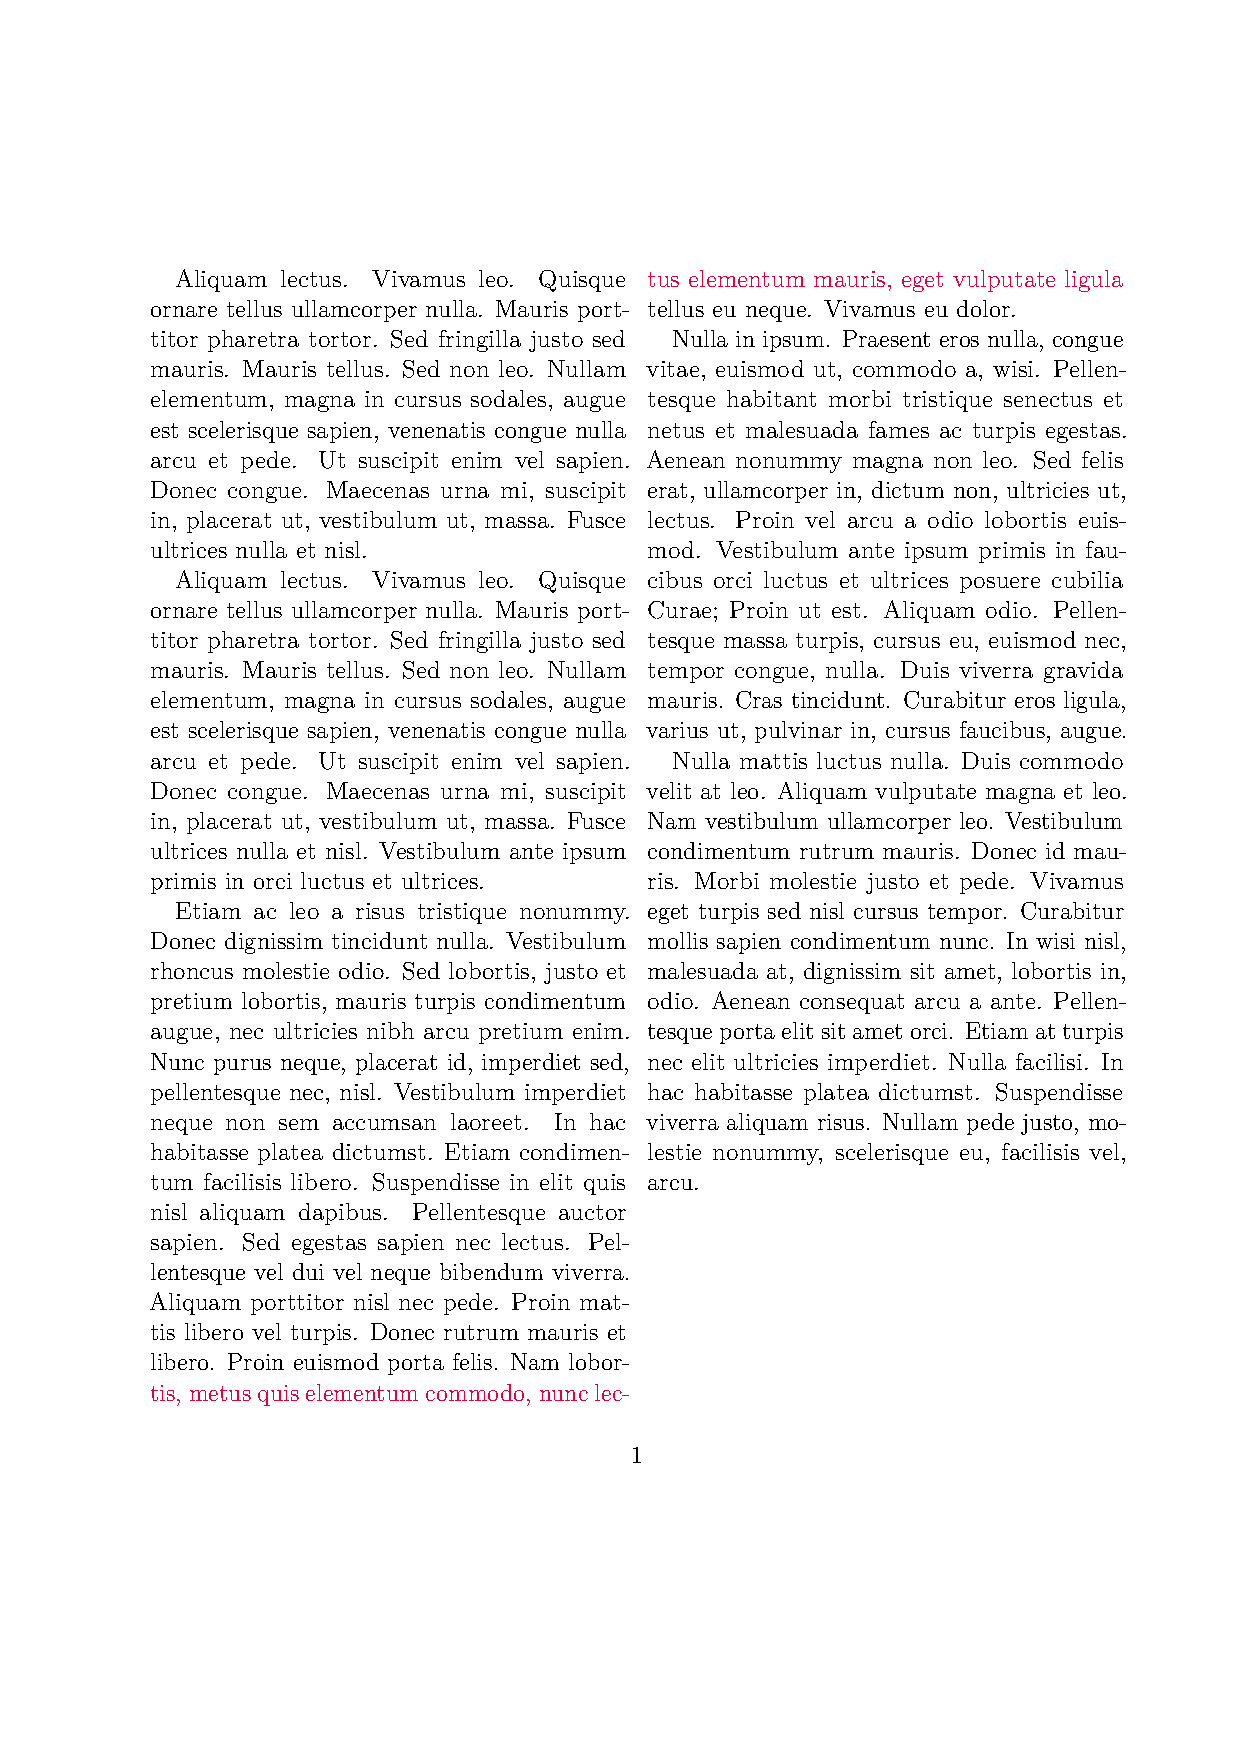
\includegraphics[height=\textheight,page=1]{examples/widow.pdf}
  \end{center}
\end{frame}

\begin{frame}
  \frametitle{Potlačený sirotek}
  \begin{center}
    \includegraphics[height=\textheight,page=2]{examples/widow.pdf}
  \end{center}
\end{frame}

\begin{frame}
  \frametitle{Porovnání různých metod k omezení parchantů}
  \begin{priklad}
  \begin{center}
  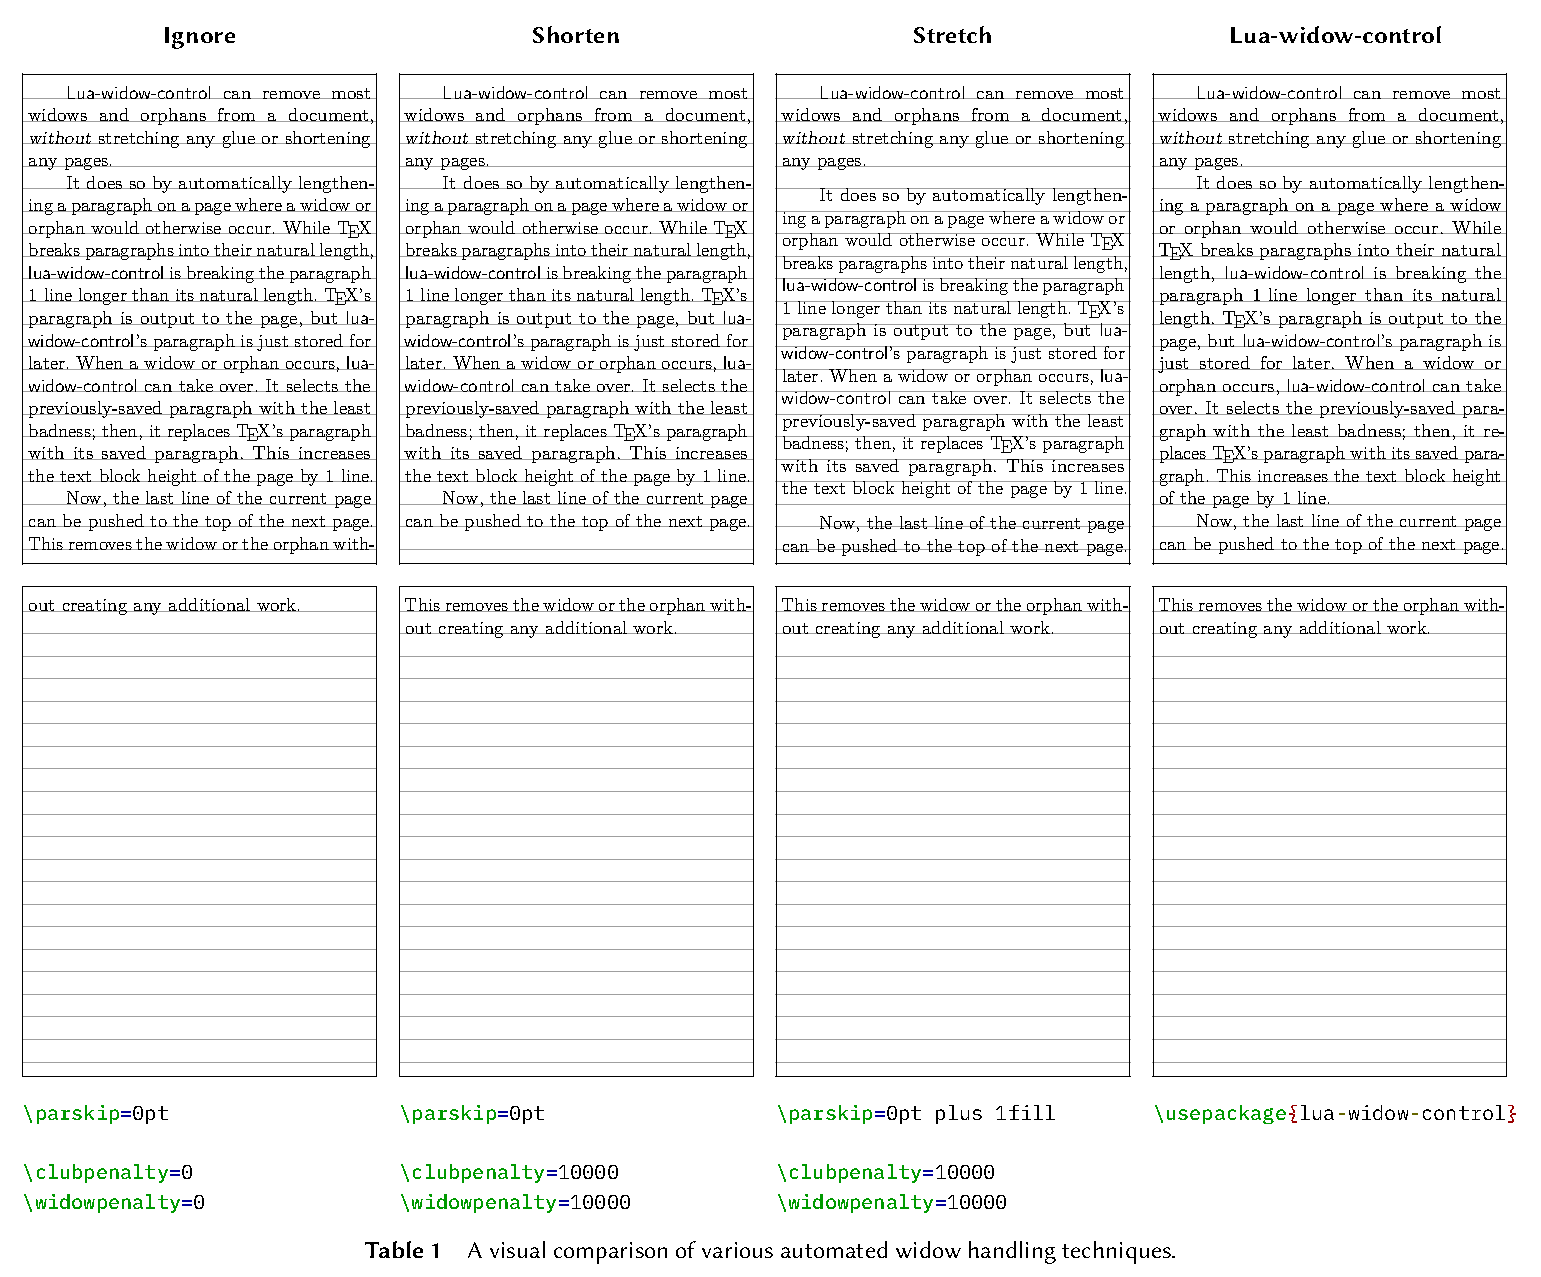
\includegraphics[height=.95\textheight]{img/lua-widow.pdf}
  \end{center}
\end{priklad}
  % \myfig[height=0.8\textheight]{img/lua-widow.pdf}{}
\end{frame}

\begin{frame}[fragile]
  \frametitle{Možnosti nastavení}
 \begin{verbatim}
 \lwcsetup{...}
 \end{verbatim}
 \begin{description}
   \item[default] -- nepřidává žádné vertikální mezery, ale může vést k příliš vzdušným odstavcům
   \item[strict] -- využívá primárně vertikální mezery a nevytváří špatné odstavce,  
     \begin{itemize}
       \item ale odstraní jen třetinu parchantů
        \item funguje špatně hlavně pro dokumenty, které obsahují jen text, beletrii apod.
      \end{itemize}
    \item[balanced] -- kombinuje obě metody, odstraní 90\% parchantů
  \end{description}
\end{frame}

\begin{frame}[fragile]
  \frametitle{Omezení}
    \begin{itemize}
      \item \verb|\clubpenalty| a \verb|\widowpenalty| nemají žádný efekt, naopak mohou způsobit vedlejší účinky
      \item  podpora pro více sloupcovou sazbu je omezená, balíček Multicol nefunguje
  \end{itemize}
\end{frame}
 

\begin{frame}[fragile]
  \frametitle{Balíček \texttt{luavlna}}
    Zamezuje rozdělení řádků:
      \begin{itemize}
        \item za jednoslovnými předložkami
        \item u iniciál
        \item u akademických titulů
        \item mezi čísly a jednotkami
      \end{itemize}
  \url{https://ctan.org/pkg/luavlna}
\end{frame}

\begin{frame}
  \frametitle{Ukázka užití Luavlny}
  \begin{minipage}{3in}

    \preventsingledebugon

    Text s krátkými souhláskami a samohláskami i dalšími jevy
    z nabídky možností (v textu možnými).

    Co třeba í znaky š diakritikou?

    Různé možnosti [v závorkách \textless i jiných znacích

    Podpora iniciál a titulů: M. J. Hegel, Ing. Běháková, Ph.D., Ž. Zíbrt,
    Ch. Borner.

    Podpora jednotek: 100,5 MN\cdot{}s, 100.5 kJ, 200 µA, $-1$ dag, 1 MB. 1 kJ.

    Uvnitř matematiky by mělo být zpracování vypnuté: $k \in \mathbb N$.

    \preventsingledebugoff
  \end{minipage}
\end{frame}

\begin{frame}
    \frametitle{Zalamování spojovníků}
    \begin{center}
    \begin{minipage}{2in}
      Sedlec-Prčice, modro-zelený, překladatel-tlumočník, kuchař-číšník, propan-butan, Otýlie Sklenářová-Malá, František Jílek-Oberpfalcer.
    \end{minipage}
  \end{center}
\end{frame}

\begin{frame}
  \frametitle{Volby balíčku}
  Pomocí voleb můžeme zakázat některé vlastnosti
  \begin{description}
    \item [noprocess] – nespouštět zpracování dokumentu automaticky
    \item [noinitials] – iniciály
    \item [nounits] – SI jednotky
    \item [nopredegrees] – tituly před jménem
    \item [nosufdegrees] – tituly za jménem
  \end{description}
\end{frame}

\begin{frame}[fragile]
  \frametitle{Užitečné příkazy}
  \begin{itemize}
    \item \verb|\singlechars{jazyk}{písmena}| -- seznam písmen, u kterých se potlačuje zalamování řádků

    \item \verb|\enablesplithyphens{jazyk}| -- nastaví podporu zalamování spojovníků pro daný jazyk
    \item \verb|\preventsinglelang{jazyk}| -- nastaví pravidla pro daný jazyk pro celý dokument
  \end{itemize}
\end{frame}

\begin{frame}[fragile]
  \frametitle{Podporované jazyky}
  Vestavěná podpora je pouze pro češtinu a slovenštinu:

\begin{verbatim}
\singlechars{czech}{AIiVvOoUuSsZzKk}
\singlechars{slovak}{AIiVvOoUuSsZzKk}
\end{verbatim}

Je třeba jazyk vybrat pomocí balíčků Babel nebo Polyglossia

\begin{verbatim}
A příklad česky.
\selectlanguage{english}
A something.
\end{verbatim}

    \preventsingledebugon

A příklad česky.
\selectlanguage{english}
A something.

    \preventsingledebugoff

    \selectlanguage{czech}

\end{frame}

\newcommand\testbox[1]{%
  \parbox{150pt}{%
    \parindent=15pt%
    \tolerance=1%
    \pretolerance=1%
    #1
  }%
}

\newcommand\printtest[1]{%
  \linebreakerdisable%
  \noindent\testbox{%
    #1
    \par\medskip\noindent\hfill\textbf{Bez Linebreakeru}\hfill\null
  }%
  \linebreakerenable%
  \hfill%
  \testbox{%
    #1
    \par\medskip\noindent\hfill\textbf{S Linebreakerem}\hfill\null
  }%
}


\begin{frame}[fragile]
  \frametitle{Balíček \texttt{linebreaker}}
  Brání výskytu přetečených řádků
  \begin{itemize}
    \item ovlivňuje pouze sazbu  odstavců, kde se takový řádek vyskytl
    \item pokud detekuje přetečený řádek v odstavci, vysází ho znovu s většími hodnotami
      \verb|tolerance| a \verb|emergencystretch|.
  \end{itemize}
  \url{https://ctan.org/pkg/linebreaker}
\end{frame}
  
\begin{frame}
  \frametitle{Příklad}
  \printtest{
    The example document given below creates two pages by using Lua code alone. You
will learn how to access TeX's boxes and counters from the Lua side, shipout a
page into the PDF file, create horizontal and vertical boxes (hbox and vbox),
create new nodes and manipulate the nodes links structure. 
%The example covers the following node types: rule, whatsit, vlist, hlist and action.
  }

\end{frame}
 
\begin{frame}[fragile]
  \frametitle{Nastavení}
  Linebreaker můžeme konfigurovat pomocí příkazu \verb|\linebreakersetup|:
  \begin{description}
    \item[maxcycles] -- počet pokusů o přesázení odstavce
    \item[maxemergencystretch] -- maximální hodnota \verb|\emergencystretch|
    \item[maxtolerance]  -- maximální hodnota \verb|tolerance|
  \end{description}
\begin{verbatim}
\linebreakersetup{
maxtolerance = 90,         % default 9999
maxemergencystretch = 1em, % default 3em
maxcycles = 4              % default 30
}
\end{verbatim}

\end{frame}

% \section{Závěr}

\begin{frame}[standout]

 
  Děkuji za pozornost!

  \url{michal.h21@gmail.com}

  \url{www.kodymirus.cz}

\end{frame}
